\chapter{Diseño del acelerador HAWK}
\label{ch:design}

\section{Estudio y selección de aceleradores criptográficos}
Previo al diseño del acelerador, se realizó un estudio 
de los esquemas de firma poscuántica que participaban en la segunda
ronda del proceso de firmas adicionales del NIST. 
En esta primera fase se realizó un análisis para su 
implementación parcial o total de los diferentes 
algoritmos propuestos.
El estudio completo se recoge en el apéndice~\ref{anexo:aceleradores}.


Para el estudio se emplearon los siguientes criterios de selección:
\begin{enumerate}
    \item Viabilidad de implementación.
    \item Complejidad de las operaciones.
    \item Consumo de recursos y memoria.
    \item Complejidad del control.
    \item Disponibilidad de implementaciones y documentación.
    \item Potencial de aceleración.
    \item Adecuación a una arquitectura hardware-software.
    \item Carga de hashing.
\end{enumerate}


El orden de preferencia de los candidatos se recoge en la
tabla~\ref{tab:eval-clasificacion} del
apéndice~\ref{anexo:aceleradores}.

Los esquemas multivariantes como UOV, consistente en la resolución de problemas matriciales,
fueron considerados inicialmente. 
Sin embargo, se descartaron por el elevado consumo de BRAM y LUT en algunas de las implementaciones revisadas.

Aunque para el esquema HAWK no se identificaron diseños totales o parciales en FPGA en la revisión realizada, 
se realizó un análisis cualitativo en función de las prestaciones necesarias para el mismo. 
Por tanto, uno de los resultados que se analizarán será la utilización de recursos del acelerador de HAWK.

HAWK se seleccionó por la ausencia de operaciones en coma flotante, reduciendo su complejidad en hardware. 
Posteriormente, se tuvieron en consideración las limitaciones existentes del SoC PYNQ-Z2.
Para esta implementación se optó por un diseño dual entre procesador y lógica programable.
En futuros capítulos se detallará la distribución de tareas en función de las prestaciones.

La selección y diseño de HAWK se realizó con anterioridad al conocimiento de la retirada de HAWK.
Sin embargo, no compromete la finalidad del proyecto ya que se busca la viabilidad de implementar
algoritmos de firma poscuántica en lógica programable frente a un diseño completo en procesador.

\section{Arquitectura general del acelerador}
\label{sec:arquitectura-acelerador}

\subsection{Alcance del acelerador}

El sistema desarrollado contempla los procesos de generación
de claves, generación de firmas y verificación de firmas
descritos en el capítulo~\ref{ch:background}.
En este capítulo se presenta la distribución de tareas
entre el procesador y la lógica programable.

El esquema criptográfico consta de tres funcionalidades:
\begin{enumerate}
    \item Generación de claves: produce una clave privada,
    que debe mantenerse secreta, y una clave pública, que puede compartirse.
    \item Generación de firmas: utiliza la clave privada
    para generar una firma asociada a un mensaje.
    \item Verificación de firmas: utiliza la clave pública
    para comprobar la validez de la firma asociada al mensaje.
    Una firma inválida se rechaza.
\end{enumerate}
Se han implementado estos tres procesos en el sistema.
A continuación se determina la gestión de tareas para cada proceso.

\subsection{Distribución de tareas}
\subsubsection{Generación de claves}

La figura~\ref{fig:hawk-keygen} reproduce el algoritmo de generación
de claves \texttt{HawkKeyGen} de la especificación de HAWK
\cite[p.~24, algoritmo~13]{hawk-spec-2025}. Sus pasos se utilizan
como referencia para describir la distribución de tareas entre
el procesador y la lógica programable.

\begin{figure}[H]
    \centering
    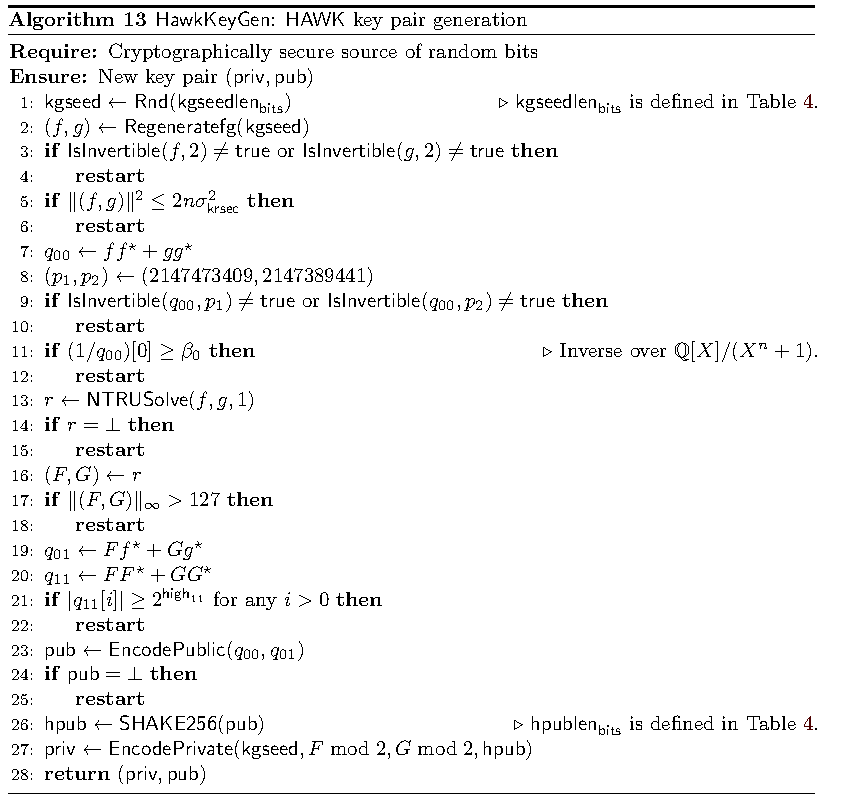
\includegraphics[width=\textwidth,height=0.73\textheight,keepaspectratio]{hawk-keygen.pdf}
    \caption{Generación del par de claves de HAWK mediante \texttt{HawkKeyGen}.
    Fuente: algoritmo 13 de la especificación de HAWK, versión 1.1
    \cite[p.~24]{hawk-spec-2025}.}
    \label{fig:hawk-keygen}
\end{figure}

En un primer análisis, se determinan las implementaciones que hay que realizar:
\begin{enumerate}
    \item Generación de una semilla aleatoria mediante una fuente criptográficamente segura (PS)
    \item Regeneración de los polinomios $f$ y $g$ a partir de la semilla (PS)
    \item Comprobación de invertibilidad (PS)
    \item Cálculo de normas y comprobación de cotas (PS)
    \item Cálculo de polinomios adjuntos (PS)
    \item Resolución de la ecuación NTRU (PS)
    \item Funciones de codificación (PS)
    \item Cálculo del hash de la clave pública mediante SHAKE256 (PS)
\end{enumerate}

La generación de claves se realiza íntegramente en el procesador. 
Cuando alguna de las comprobaciones falla, 
el algoritmo descarta el candidato y reinicia el proceso. 
Esto introduce un número variable de iteraciones y 
complica el control de una implementación en lógica programable. 
Por ello, se reservan los recursos lógicos disponibles 
para acelerar la firma y la verificación.

\subsubsection{Generación de la firma}

La figura~\ref{fig:hawk-sign} reproduce el algoritmo de generación
de firmas \texttt{HawkSign} de la especificación de HAWK
\cite[p.~28, algoritmo~15]{hawk-spec-2025}. Sus pasos se utilizan
como referencia para describir la distribución de tareas entre
el procesador y la lógica programable.

\begin{figure}[H]
    \centering
    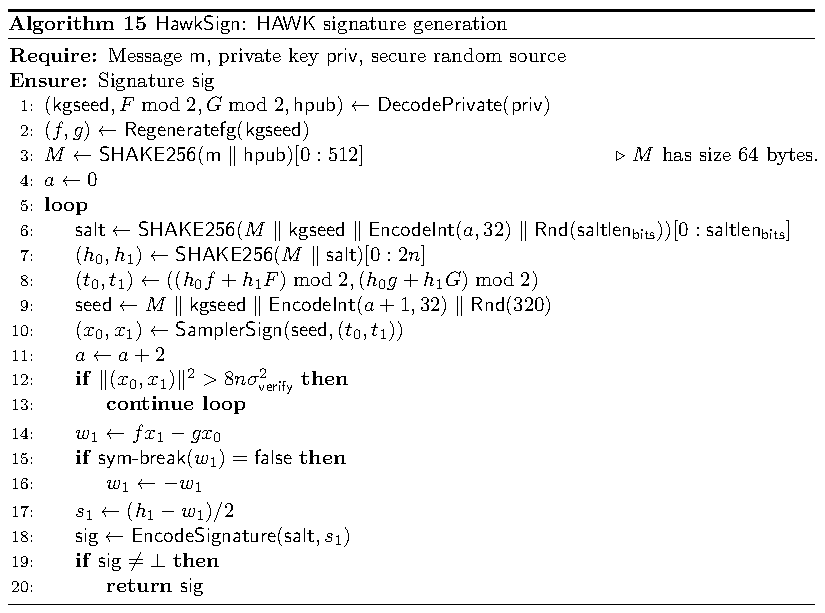
\includegraphics[width=\textwidth,height=0.73\textheight,keepaspectratio]{hawk-sign.pdf}
    \caption{Generación de una firma HAWK mediante \texttt{HawkSign}.
    Fuente: algoritmo 15 de la especificación de HAWK, versión 1.1
    \cite[p.~28]{hawk-spec-2025}.}
    \label{fig:hawk-sign}
\end{figure}

En un primer análisis se determinan las implementaciones que hay que realizar:
\begin{enumerate}
    \item Decodificación de clave privada (PS)
    \item Regeneración de los polinomios $f$ y $g$ a partir de la semilla (PS)
    \item Cálculo de $M$ mediante SHAKE256 sobre la concatenación del mensaje y el hash de la clave pública (PS)
    \item Generación de \texttt{salt} mediante SHAKE256 (PS)
    \item Generación de $h_0$ y $h_1$ mediante SHAKE256 (PS)
    \item Cálculo de $t_0$ y $t_1$ a partir de polinomios binarios (PL)
    \item Generación de la semilla y muestreo de los polinomios $x_0$ y $x_1$ mediante \texttt{SamplerSign} (PS)
    \item Cálculo y comprobación de la norma (PS)
    \item Cálculo de $w_1$ (PL)
    \item Comprobación de \texttt{sym-break} (PL)
    \item Cálculo de $s_1$ (PL)
    \item Cálculo de la firma mediante codificación de $s_1$ y \texttt{salt} (PS)
\end{enumerate}

Para la generación de firmas, se ejecutan en lógica programable los cálculos
de los polinomios $t_0$, $t_1$, $w_1$ y $s_1$ así como la comprobación y corrección
de la ruptura de simetría. Por otra parte, el procesador realiza las tareas de
codificación, hashing, muestreo y generación de variables aleatorias así como
la comprobación de la norma. Esta distribución permite acelerar las operaciones aritméticas
mediante el uso de recursos DSP de la lógica programable.

El algoritmo repite el intento cuando la norma supera la cota establecida
o cuando falla la codificación de la firma. 
En ambos casos, vuelve a la generación de \texttt{salt}, 
sin repetir la decodificación de la clave privada 
ni la regeneración de los polinomios $f$ y $g$.

\subsubsection{Verificación de la firma}

La figura~\ref{fig:hawk-verify} reproduce el algoritmo de verificación
de firmas \texttt{HawkVerify} de la especificación de HAWK
\cite[p.~36, algoritmo~20]{hawk-spec-2025}. Sus pasos se utilizan
como referencia para describir la distribución de tareas entre
el procesador y la lógica programable.

\begin{figure}[H]
    \centering
    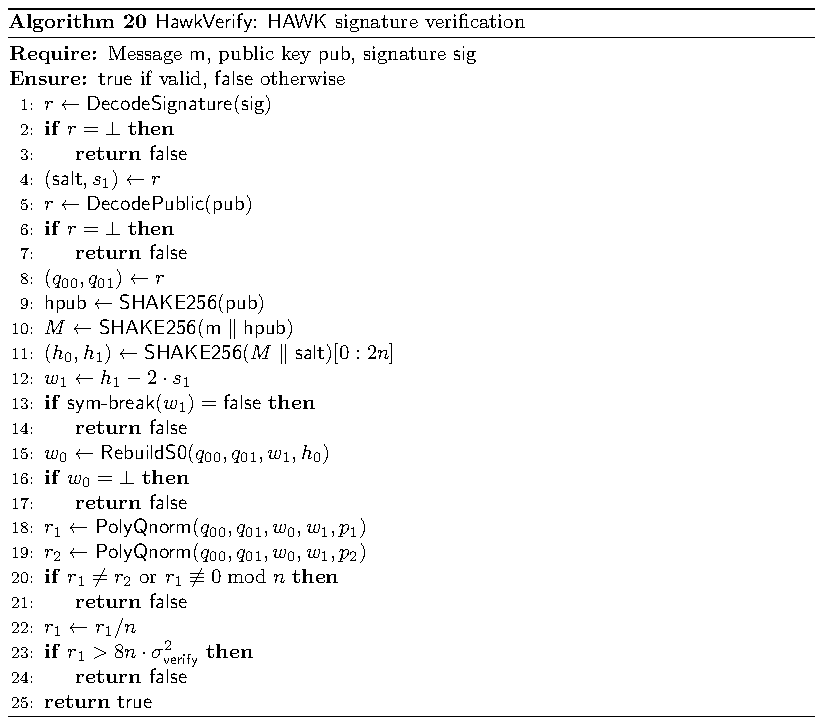
\includegraphics[width=\textwidth,height=0.73\textheight,keepaspectratio]{hawk-verify.pdf}
    \caption{Verificación de una firma HAWK mediante \texttt{HawkVerify}.
    Fuente: algoritmo 20 de la especificación de HAWK, versión 1.1
    \cite[p.~36]{hawk-spec-2025}.}
    \label{fig:hawk-verify}
\end{figure}

En un primer análisis se determinan las implementaciones que hay que realizar:
\begin{enumerate}
    \item Decodificación de la firma y la clave pública (PS)
    \item Cálculo de hash de la clave pública mediante SHAKE256 (PS)
    \item Cálculo de $M$ mediante SHAKE256 sobre la concatenación del mensaje y el hash de la clave pública (PS)
    \item Generación de $h_0$ y $h_1$ mediante SHAKE256 (PS)
    \item Cálculo de $w_1$ (PS)
    \item Comprobación de \texttt{sym-break} (PL)
    \item Cálculo de $w_0$ mediante \texttt{RebuildS0} (PL)
    \item Cálculo de $r_1$ y $r_2$ mediante \texttt{PolyQNorm} (PL)
    \item Comprobación de igualdad entre $r_1$ y $r_2$ y de divisibilidad de $r_1$ entre $n$ (PL)
    \item Comparación de $r_1/n$ con la cota superior (PL)
\end{enumerate}

Para la verificación de la firma se distribuyeron las tareas análogamente
a la generación de firmas. Los principales cálculos aritméticos
se realizan en lógica programable mientras que las codificaciones, decodificaciones
y cálculos de hash se realizan en el procesador. El cálculo de $w_1$ se realizó
en procesador para reducir el movimiento de datos entre procesador y
lógica programable.

En este caso, no se da ninguna condición para tener que reiniciar el procesamiento
en caso de error. Se reporta al procesador si la firma es válida o no según el
resultado de las operaciones.

\subsection{Arquitectura del sistema}

En esta sección se describen los elementos que conforman la arquitectura
general del sistema, la interfaz de comunicación empleada y la gestión de tareas.

La figura~\ref{fig:diagrama-bloques-hawk} muestra el diagrama de bloques
del sistema, que integra el procesador Zynq, el acelerador HAWK,
el controlador DMA y las interconexiones AXI.

\begin{figure}[H]
    \centering
    \begingroup
    \setlength{\unitlength}{0.000534188\textwidth}
    \linethickness{1pt}
    \begin{picture}(1872,288)
        \put(0,0){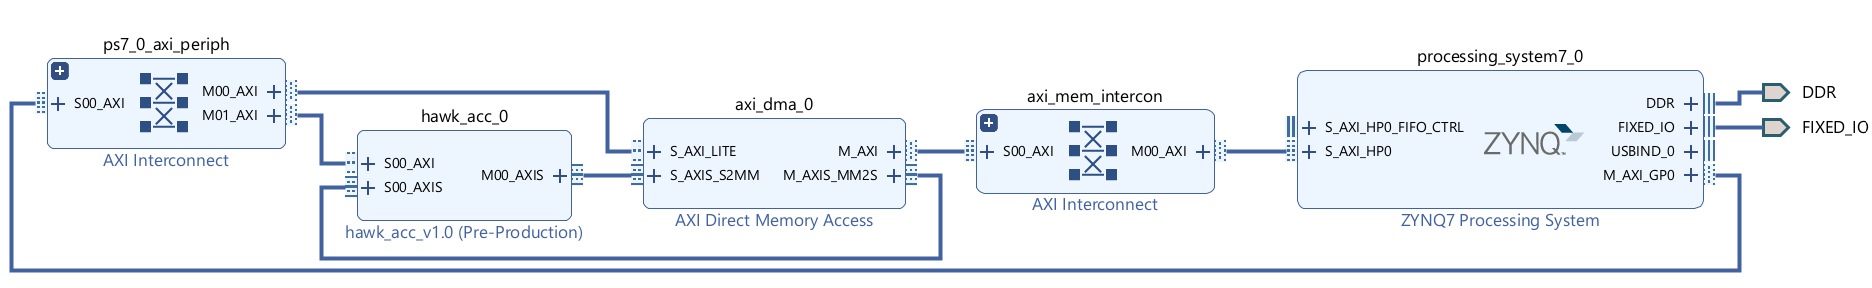
\includegraphics[width=\textwidth]{diagrama-bloques-hawk.png}}
        \color{violet}\put(44,113){\framebox(245,144){}}
        \color{orange!85!black}\put(345,40){\framebox(239,150){}}
        \color{teal}\put(636,53){\framebox(278,148){}}
        \color{magenta}\put(969,69){\framebox(253,140){}}
        \color{blue}\put(1289,51){\framebox(422,199){}}
    \end{picture}
    \endgroup
    \par\smallskip
    {\small
    \textcolor{violet}{\textbf{1. Interconexión de control}}\quad
    \textcolor{orange!85!black}{\textbf{2. Acelerador HAWK}}\quad
    \textcolor{teal}{\textbf{3. DMA}}\par
    \textcolor{magenta}{\textbf{4. Interconexión de memoria}}\quad
    \textcolor{blue}{\textbf{5. Sistema de procesamiento Zynq}}\par}
    \caption{Diagrama de bloques del sistema de aceleración de HAWK en Vivado.}
    \label{fig:diagrama-bloques-hawk}
\end{figure}

El sistema consta de los siguientes componentes:
\begin{enumerate}
    \item Sistema de procesamiento Zynq: Ejecuta las funciones de software del acelerador,
    inicia las transferencias de datos, configura las IP y escribe y lee registros de la lógica programable.
    \item Acelerador HAWK: Implementa la lógica programable del acelerador HAWK para la firma
    y verificación de la firma. Controla el camino de datos y el camino de control.
    \item DMA: Realiza las transferencias de datos entre la memoria DDR y el acelerador.
    El canal MM2S lee datos de memoria y los envía al acelerador. 
    El canal S2MM recibe los datos del acelerador y los escribe en memoria.
    \item Interconexiones: Proporcionan los canales de comunicación para el control y transferencia de datos.
    Hay dos interconexiones. La interconexión de control permite al procesador comunicarse
    con los registros del DMA y el acelerador. 
    La interconexión de memoria conecta el DMA con el sistema de procesamiento para acceder a la memoria DDR.
\end{enumerate}

En el proceso de generación de claves no interviene el DMA, ya que
el procesamiento se realiza únicamente en PS. 
Para la firma y la verificación intervienen el PS y la PL, con el siguiente flujo general:
\begin{enumerate}
    \item El procesador configura el acelerador y el DMA
    \item El procesador inicia las transferencias necesarias
    mediante los canales MM2S y, cuando corresponde, S2MM.
    \item El DMA transfiere los datos entre la memoria DDR
    y el acelerador.
    \item El procesador comprueba la finalización de las
    transferencias y de la operación.
\end{enumerate}